\documentclass[twoside]{book}

% Packages required by doxygen
\usepackage{fixltx2e}
\usepackage{calc}
\usepackage{doxygen}
\usepackage[export]{adjustbox} % also loads graphicx
\usepackage{graphicx}
\usepackage[utf8]{inputenc}
\usepackage{makeidx}
\usepackage{multicol}
\usepackage{multirow}
\PassOptionsToPackage{warn}{textcomp}
\usepackage{textcomp}
\usepackage[nointegrals]{wasysym}
\usepackage[table]{xcolor}

% Font selection
\usepackage[T1]{fontenc}
\usepackage[scaled=.90]{helvet}
\usepackage{courier}
\usepackage{amssymb}
\usepackage{sectsty}
\renewcommand{\familydefault}{\sfdefault}
\allsectionsfont{%
  \fontseries{bc}\selectfont%
  \color{darkgray}%
}
\renewcommand{\DoxyLabelFont}{%
  \fontseries{bc}\selectfont%
  \color{darkgray}%
}
\newcommand{\+}{\discretionary{\mbox{\scriptsize$\hookleftarrow$}}{}{}}

% Page & text layout
\usepackage{geometry}
\geometry{%
  a4paper,%
  top=2.5cm,%
  bottom=2.5cm,%
  left=2.5cm,%
  right=2.5cm%
}
\tolerance=750
\hfuzz=15pt
\hbadness=750
\setlength{\emergencystretch}{15pt}
\setlength{\parindent}{0cm}
\setlength{\parskip}{3ex plus 2ex minus 2ex}
\makeatletter
\renewcommand{\paragraph}{%
  \@startsection{paragraph}{4}{0ex}{-1.0ex}{1.0ex}{%
    \normalfont\normalsize\bfseries\SS@parafont%
  }%
}
\renewcommand{\subparagraph}{%
  \@startsection{subparagraph}{5}{0ex}{-1.0ex}{1.0ex}{%
    \normalfont\normalsize\bfseries\SS@subparafont%
  }%
}
\makeatother

% Headers & footers
\usepackage{fancyhdr}
\pagestyle{fancyplain}
\fancyhead[LE]{\fancyplain{}{\bfseries\thepage}}
\fancyhead[CE]{\fancyplain{}{}}
\fancyhead[RE]{\fancyplain{}{\bfseries\leftmark}}
\fancyhead[LO]{\fancyplain{}{\bfseries\rightmark}}
\fancyhead[CO]{\fancyplain{}{}}
\fancyhead[RO]{\fancyplain{}{\bfseries\thepage}}
\fancyfoot[LE]{\fancyplain{}{}}
\fancyfoot[CE]{\fancyplain{}{}}
\fancyfoot[RE]{\fancyplain{}{\bfseries\scriptsize Generated by Doxygen }}
\fancyfoot[LO]{\fancyplain{}{\bfseries\scriptsize Generated by Doxygen }}
\fancyfoot[CO]{\fancyplain{}{}}
\fancyfoot[RO]{\fancyplain{}{}}
\renewcommand{\footrulewidth}{0.4pt}
\renewcommand{\chaptermark}[1]{%
  \markboth{#1}{}%
}
\renewcommand{\sectionmark}[1]{%
  \markright{\thesection\ #1}%
}

% Indices & bibliography
\usepackage{natbib}
\usepackage[titles]{tocloft}
\setcounter{tocdepth}{3}
\setcounter{secnumdepth}{5}
\makeindex

% Hyperlinks (required, but should be loaded last)
\usepackage{ifpdf}
\ifpdf
  \usepackage[pdftex,pagebackref=true]{hyperref}
\else
  \usepackage[ps2pdf,pagebackref=true]{hyperref}
\fi
\hypersetup{%
  colorlinks=true,%
  linkcolor=blue,%
  citecolor=blue,%
  unicode%
}

% Custom commands
\newcommand{\clearemptydoublepage}{%
  \newpage{\pagestyle{empty}\cleardoublepage}%
}

\usepackage{caption}
\captionsetup{labelsep=space,justification=centering,font={bf},singlelinecheck=off,skip=4pt,position=top}

%===== C O N T E N T S =====

\begin{document}

% Titlepage & ToC
\hypersetup{pageanchor=false,
             bookmarksnumbered=true,
             pdfencoding=unicode
            }
\pagenumbering{roman}
\begin{titlepage}
\vspace*{7cm}
\begin{center}%
{\Large My Project }\\
\vspace*{1cm}
{\large Generated by Doxygen 1.8.11}\\
\end{center}
\end{titlepage}
\clearemptydoublepage
\tableofcontents
\clearemptydoublepage
\pagenumbering{arabic}
\hypersetup{pageanchor=true}

%--- Begin generated contents ---
\chapter{Namespace Index}
\section{Packages}
Here are the packages with brief descriptions (if available)\+:\begin{DoxyCompactList}
\item\contentsline{section}{\hyperlink{namespacepyexample}{pyexample} \\*Documentation for this module }{\pageref{namespacepyexample}}{}
\end{DoxyCompactList}

\chapter{Hierarchical Index}
\section{Class Hierarchy}
This inheritance list is sorted roughly, but not completely, alphabetically\+:\begin{DoxyCompactList}
\item Move\+Group\+Commander\begin{DoxyCompactList}
\item \contentsline{section}{ms\+Move\+Group.\+ms\+Move\+Group}{\pageref{classmsMoveGroup_1_1msMoveGroup}}{}
\item \contentsline{section}{ms\+Move\+Group\+Old.\+ms\+Move\+Group}{\pageref{classmsMoveGroupOld_1_1msMoveGroup}}{}
\end{DoxyCompactList}
\item \contentsline{section}{ms\+Math.\+online\+Standard\+Deviations}{\pageref{classmsMath_1_1onlineStandardDeviations}}{}
\item \contentsline{section}{ms\+Tf\+Getter.\+tf\+Getter}{\pageref{classmsTfGetter_1_1tfGetter}}{}
\end{DoxyCompactList}

\chapter{Class Index}
\section{Class List}
Here are the classes, structs, unions and interfaces with brief descriptions\+:\begin{DoxyCompactList}
\item\contentsline{section}{\hyperlink{classkondoServoLib_1_1b3mCtrl_07_xE3_x82_xB3_xE3_x83_x94_xE3_x83_xBC_08_1_1B3mClass}{kondo\+Servo\+Lib.\+b3m\+Ctrl(コピー).\+B3m\+Class} }{\pageref{classkondoServoLib_1_1b3mCtrl_07_xE3_x82_xB3_xE3_x83_x94_xE3_x83_xBC_08_1_1B3mClass}}{}
\item\contentsline{section}{\hyperlink{classkondoServoLib_1_1b3mCtrl_1_1B3mClass}{kondo\+Servo\+Lib.\+b3m\+Ctrl.\+B3m\+Class} }{\pageref{classkondoServoLib_1_1b3mCtrl_1_1B3mClass}}{}
\item\contentsline{section}{\hyperlink{classkondoServoLib_1_1ctrlKondoServo_1_1ctrlKondoServoClass}{kondo\+Servo\+Lib.\+ctrl\+Kondo\+Servo.\+ctrl\+Kondo\+Servo\+Class} }{\pageref{classkondoServoLib_1_1ctrlKondoServo_1_1ctrlKondoServoClass}}{}
\item\contentsline{section}{\hyperlink{classkondoServoLib_1_1icsCtrl_1_1IcsClass}{kondo\+Servo\+Lib.\+ics\+Ctrl.\+Ics\+Class} }{\pageref{classkondoServoLib_1_1icsCtrl_1_1IcsClass}}{}
\end{DoxyCompactList}

\chapter{Namespace Documentation}
\hypertarget{namespacepyexample}{}\section{pyexample Namespace Reference}
\label{namespacepyexample}\index{pyexample@{pyexample}}


Documentation for this module.  




\subsection{Detailed Description}
Documentation for this module. 

More details. \begin{DoxyAuthor}{Author}
sugino 
\end{DoxyAuthor}
\begin{DoxyVersion}{Version}
1.\+1 
\end{DoxyVersion}
\begin{DoxySince}{Since}
2019/02/02 
\end{DoxySince}

\chapter{Class Documentation}
\hypertarget{classmsMoveGroup_1_1msMoveGroup}{}\section{ms\+Move\+Group.\+ms\+Move\+Group Class Reference}
\label{classmsMoveGroup_1_1msMoveGroup}\index{ms\+Move\+Group.\+ms\+Move\+Group@{ms\+Move\+Group.\+ms\+Move\+Group}}


rosのmove\+\_\+groupクラスを継承して、いくつか関数を追加したもの~\newline
  




Inheritance diagram for ms\+Move\+Group.\+ms\+Move\+Group\+:\nopagebreak
\begin{figure}[H]
\begin{center}
\leavevmode
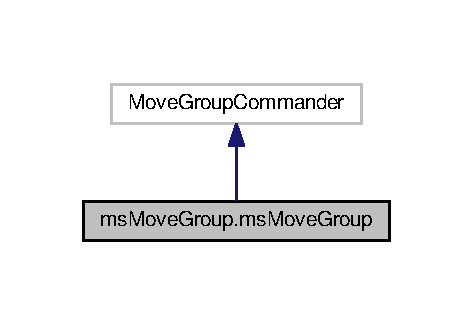
\includegraphics[width=227pt]{classmsMoveGroup_1_1msMoveGroup__inherit__graph}
\end{center}
\end{figure}


Collaboration diagram for ms\+Move\+Group.\+ms\+Move\+Group\+:\nopagebreak
\begin{figure}[H]
\begin{center}
\leavevmode
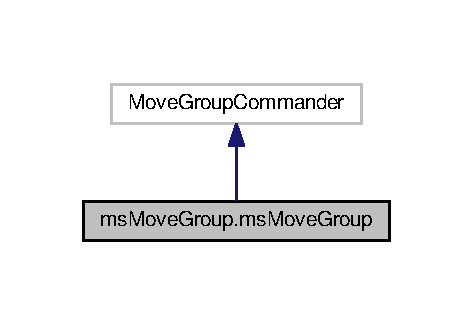
\includegraphics[width=227pt]{classmsMoveGroup_1_1msMoveGroup__coll__graph}
\end{center}
\end{figure}
\subsection*{Public Member Functions}
\begin{DoxyCompactItemize}
\item 
def \hyperlink{classmsMoveGroup_1_1msMoveGroup_a9800d2afd662bf45ccfb978007a55f08}{\+\_\+\+\_\+init\+\_\+\+\_\+} (self, group\+Name)
\item 
def \hyperlink{classmsMoveGroup_1_1msMoveGroup_aadc2635eb78a0043d4f30ecc30eae959}{ms\+Plan} (self, kwargs)
\begin{DoxyCompactList}\small\item\em 軌道を生成する~\newline
 優先順位\+: random $>$ pose\+Name $>$ joint $>$ pose $>$ position $>$ posture ~\newline
 例)ms\+Plan(joint=\mbox{[}0,0,0,0,0,0\mbox{]}) \end{DoxyCompactList}\item 
def \hyperlink{classmsMoveGroup_1_1msMoveGroup_aa3914f9104f9459d971f10d49fbf2d62}{ms\+Go} (self, kwargs)
\begin{DoxyCompactList}\small\item\em 軌跡の計画と実行を行う。計画(plan)を渡すと実行のみを行う~\newline
 優先順位\+: plan $>$ random $>$ pose\+Name $>$ joint $>$ pose $>$ position $>$ posture ~\newline
 例)ms\+Go(joint=\mbox{[}0,0,0,0,0,0\mbox{]}) \end{DoxyCompactList}\item 
def \hyperlink{classmsMoveGroup_1_1msMoveGroup_a3261620111e34668e764c0d522794b3a}{ms\+Plan\+Way} (self, way\+Point, eef\+\_\+step=0.\+01, jump\+\_\+threshold=0.\+0, avoid\+\_\+collisions=True, move\+Success\+Ratio=0.\+5)\hypertarget{classmsMoveGroup_1_1msMoveGroup_a3261620111e34668e764c0d522794b3a}{}\label{classmsMoveGroup_1_1msMoveGroup_a3261620111e34668e764c0d522794b3a}

\begin{DoxyCompactList}\small\item\em 最終地点までの軌跡を生成してからでなく、1ステップ先ずつ関節角度を生成するから、行き詰まりやすい \end{DoxyCompactList}\item 
def \hyperlink{classmsMoveGroup_1_1msMoveGroup_a5a35e7ca351f7d6ae9a6f8a78091061d}{ms\+Plan\+Shift} (self, vector\+List, reference\+Frame=None)
\begin{DoxyCompactList}\small\item\em reference\+Frameを基準座標としたvector\+Listの方向にエンドエフェクタを動かす軌跡を生成する \end{DoxyCompactList}\item 
def \hyperlink{classmsMoveGroup_1_1msMoveGroup_a77ea08da7914e81740daa8a35cf8bf69}{ms\+Get\+Current\+Pose} (self)\hypertarget{classmsMoveGroup_1_1msMoveGroup_a77ea08da7914e81740daa8a35cf8bf69}{}\label{classmsMoveGroup_1_1msMoveGroup_a77ea08da7914e81740daa8a35cf8bf69}

\begin{DoxyCompactList}\small\item\em reference\+Frameからみたend\+Effectorの\+Poseを取得 ~\newline
 get\+\_\+current\+\_\+poseでは、planning\+\_\+frameからの座標を取得するため \end{DoxyCompactList}\item 
def \hyperlink{classmsMoveGroup_1_1msMoveGroup_a6d54897d1d6dde1a6782da893e281609}{ms\+Point\+To\+Position} (self, goal\+Position, arm\+Position, tip\+Direction\+Vector3=\mbox{[}0, base\+Open\+Vector=\mbox{[}0)
\begin{DoxyCompactList}\small\item\em アームを何かの方向に向けたいときの姿勢を決定する関数 \end{DoxyCompactList}\item 
def \hyperlink{classmsMoveGroup_1_1msMoveGroup_afbe74bb02250901bedb872f2ca6ae542}{ms\+Pick} (self, object\+Id, gripping\+Joint\+Angle, openning\+Joint\+Angle, object\+Point=None, grip\+Posture=None, grip\+Position=\mbox{[}0, to\+Grip\+Move\+Vector=\mbox{[}0, to\+Retreat\+Move\+Vector=\mbox{[}0, try\+Num=2)
\begin{DoxyCompactList}\small\item\em 不具合あり \end{DoxyCompactList}\item 
def \hyperlink{classmsMoveGroup_1_1msMoveGroup_a203c6ca35199220d7aa82128fb50c28d}{ms\+Place} (self, object\+Id, openning\+Joint\+Angle, place\+Position, to\+Place\+Move\+Vector=\mbox{[}0, to\+Retreat\+Move\+Vector=\mbox{[}0)\hypertarget{classmsMoveGroup_1_1msMoveGroup_a203c6ca35199220d7aa82128fb50c28d}{}\label{classmsMoveGroup_1_1msMoveGroup_a203c6ca35199220d7aa82128fb50c28d}

\begin{DoxyCompactList}\small\item\em 不具合あり \end{DoxyCompactList}\item 
def {\bfseries make\+Gripper\+Posture} (self, joint\+Angle)\hypertarget{classmsMoveGroup_1_1msMoveGroup_a1bba0e1fe93c0a8306b8fbc52fc382e8}{}\label{classmsMoveGroup_1_1msMoveGroup_a1bba0e1fe93c0a8306b8fbc52fc382e8}

\item 
def {\bfseries make\+Gripper\+Translation} (self, min\+\_\+dist, desired, vector)\hypertarget{classmsMoveGroup_1_1msMoveGroup_ad1a287ac761df1eb05d97efd5bb6ac28}{}\label{classmsMoveGroup_1_1msMoveGroup_ad1a287ac761df1eb05d97efd5bb6ac28}

\item 
def \hyperlink{classmsMoveGroup_1_1msMoveGroup_af0b43285c3f86890835cfdb2bd68b9ee}{make\+Arm\+Poses} (self, position, option=\char`\"{}R\+I\+NG\char`\"{})
\item 
def \hyperlink{classmsMoveGroup_1_1msMoveGroup_a5faf711fd580658280b0611969a3c45d}{hoge} (a=\mbox{[}1)
\begin{DoxyCompactList}\small\item\em func setumei \end{DoxyCompactList}\end{DoxyCompactItemize}


\subsection{Detailed Description}
rosのmove\+\_\+groupクラスを継承して、いくつか関数を追加したもの~\newline
 

\begin{DoxyAuthor}{Author}
sugino 
\end{DoxyAuthor}
\begin{DoxyVersion}{Version}
1.\+1 
\end{DoxyVersion}
\begin{DoxySince}{Since}
2018/12/22 
\end{DoxySince}


\subsection{Constructor \& Destructor Documentation}
\index{ms\+Move\+Group\+::ms\+Move\+Group@{ms\+Move\+Group\+::ms\+Move\+Group}!\+\_\+\+\_\+init\+\_\+\+\_\+@{\+\_\+\+\_\+init\+\_\+\+\_\+}}
\index{\+\_\+\+\_\+init\+\_\+\+\_\+@{\+\_\+\+\_\+init\+\_\+\+\_\+}!ms\+Move\+Group\+::ms\+Move\+Group@{ms\+Move\+Group\+::ms\+Move\+Group}}
\subsubsection[{\texorpdfstring{\+\_\+\+\_\+init\+\_\+\+\_\+(self, group\+Name)}{__init__(self, groupName)}}]{\setlength{\rightskip}{0pt plus 5cm}def ms\+Move\+Group.\+ms\+Move\+Group.\+\_\+\+\_\+init\+\_\+\+\_\+ (
\begin{DoxyParamCaption}
\item[{}]{self, }
\item[{}]{group\+Name}
\end{DoxyParamCaption}
)}\hypertarget{classmsMoveGroup_1_1msMoveGroup_a9800d2afd662bf45ccfb978007a55f08}{}\label{classmsMoveGroup_1_1msMoveGroup_a9800d2afd662bf45ccfb978007a55f08}

\begin{DoxyParams}{Parameters}
{\em group\+Name} & Moveitで登録したグループ名 \\
\hline
\end{DoxyParams}


\subsection{Member Function Documentation}
\index{ms\+Move\+Group\+::ms\+Move\+Group@{ms\+Move\+Group\+::ms\+Move\+Group}!hoge@{hoge}}
\index{hoge@{hoge}!ms\+Move\+Group\+::ms\+Move\+Group@{ms\+Move\+Group\+::ms\+Move\+Group}}
\subsubsection[{\texorpdfstring{hoge(a=[1)}{hoge(a=[1)}}]{\setlength{\rightskip}{0pt plus 5cm}def ms\+Move\+Group.\+ms\+Move\+Group.\+hoge (
\begin{DoxyParamCaption}
\item[{}]{a = {\ttfamily \mbox{[}1}}
\end{DoxyParamCaption}
)}\hypertarget{classmsMoveGroup_1_1msMoveGroup_a5faf711fd580658280b0611969a3c45d}{}\label{classmsMoveGroup_1_1msMoveGroup_a5faf711fd580658280b0611969a3c45d}


func setumei 


\begin{DoxyParams}{Parameters}
{\em a} & print to terminal \\
\hline
\end{DoxyParams}
\index{ms\+Move\+Group\+::ms\+Move\+Group@{ms\+Move\+Group\+::ms\+Move\+Group}!make\+Arm\+Poses@{make\+Arm\+Poses}}
\index{make\+Arm\+Poses@{make\+Arm\+Poses}!ms\+Move\+Group\+::ms\+Move\+Group@{ms\+Move\+Group\+::ms\+Move\+Group}}
\subsubsection[{\texorpdfstring{make\+Arm\+Poses(self, position, option=""R\+I\+NG"")}{makeArmPoses(self, position, option="RING")}}]{\setlength{\rightskip}{0pt plus 5cm}def ms\+Move\+Group.\+ms\+Move\+Group.\+make\+Arm\+Poses (
\begin{DoxyParamCaption}
\item[{}]{self, }
\item[{}]{position, }
\item[{}]{option = {\ttfamily \char`\"{}RING\char`\"{}}}
\end{DoxyParamCaption}
)}\hypertarget{classmsMoveGroup_1_1msMoveGroup_af0b43285c3f86890835cfdb2bd68b9ee}{}\label{classmsMoveGroup_1_1msMoveGroup_af0b43285c3f86890835cfdb2bd68b9ee}

\begin{DoxyParams}{Parameters}
{\em position} & 目標(中心)位置 \\
\hline
{\em option} & \char`\"{}\+R\+I\+N\+G\char`\"{} z軸周りに円状30箇所の姿勢を生成 ~\newline
 \char`\"{}\+S\+P\+H\+E\+R\+E\char`\"{} 球状26箇所の姿勢を生成 ~\newline
 \char`\"{}\+U\+P\+P\+E\+R\+\_\+\+H\+E\+M\+I\+S\+P\+H\+E\+R\+E\char`\"{} z軸に垂直な平面で割った半球状17箇所の姿勢を生成 \\
\hline
\end{DoxyParams}
\begin{DoxyReturn}{Returns}
位置+姿勢のリスト(list\+\_\+of\+\_\+\+Pose) 
\end{DoxyReturn}
\index{ms\+Move\+Group\+::ms\+Move\+Group@{ms\+Move\+Group\+::ms\+Move\+Group}!ms\+Go@{ms\+Go}}
\index{ms\+Go@{ms\+Go}!ms\+Move\+Group\+::ms\+Move\+Group@{ms\+Move\+Group\+::ms\+Move\+Group}}
\subsubsection[{\texorpdfstring{ms\+Go(self, kwargs)}{msGo(self, kwargs)}}]{\setlength{\rightskip}{0pt plus 5cm}def ms\+Move\+Group.\+ms\+Move\+Group.\+ms\+Go (
\begin{DoxyParamCaption}
\item[{}]{self, }
\item[{}]{kwargs}
\end{DoxyParamCaption}
)}\hypertarget{classmsMoveGroup_1_1msMoveGroup_aa3914f9104f9459d971f10d49fbf2d62}{}\label{classmsMoveGroup_1_1msMoveGroup_aa3914f9104f9459d971f10d49fbf2d62}


軌跡の計画と実行を行う。計画(plan)を渡すと実行のみを行う~\newline
 優先順位\+: plan $>$ random $>$ pose\+Name $>$ joint $>$ pose $>$ position $>$ posture ~\newline
 例)ms\+Go(joint=\mbox{[}0,0,0,0,0,0\mbox{]}) 


\begin{DoxyParams}{Parameters}
{\em position(list\+\_\+of\+\_\+xyz\+\_\+position,Point,Vector3)} & = 位置 \\
\hline
{\em posture(list\+\_\+of\+\_\+xyzw,list\+\_\+of\+\_\+rpy,Quaternion)} & = 姿勢 \\
\hline
{\em pose(list\+\_\+of\+\_\+xyzxyzw,list\+\_\+of\+\_\+xyzrpy,Pose,Pose\+Stamped)} & = 位置+姿勢 \\
\hline
{\em joint(list\+\_\+of\+\_\+joints,Joint\+State)} & = 関節角度 \\
\hline
{\em pose\+Name(\+String)} & = 登録した関節角度の名前 \\
\hline
{\em random(bool)} & = 目標値をランダムに設定するか \\
\hline
{\em start\+Joint(list\+\_\+of\+\_\+joints,Joint\+State,Robot\+State)} & = 計画を作る初期の関節の状態 \\
\hline
{\em plan(\+Robot\+Trajectory)} & = 事前に立てた計画 \\
\hline
{\em is\+Wait\+Display\+Rviz(bool)} & = Rvizの描画完了まで待つかどうか \\
\hline
\end{DoxyParams}
\begin{DoxyReturn}{Returns}
成否(bool) 
\end{DoxyReturn}
\index{ms\+Move\+Group\+::ms\+Move\+Group@{ms\+Move\+Group\+::ms\+Move\+Group}!ms\+Pick@{ms\+Pick}}
\index{ms\+Pick@{ms\+Pick}!ms\+Move\+Group\+::ms\+Move\+Group@{ms\+Move\+Group\+::ms\+Move\+Group}}
\subsubsection[{\texorpdfstring{ms\+Pick(self, object\+Id, gripping\+Joint\+Angle, openning\+Joint\+Angle, object\+Point=\+None, grip\+Posture=\+None, grip\+Position=[0, to\+Grip\+Move\+Vector=[0, to\+Retreat\+Move\+Vector=[0, try\+Num=2)}{msPick(self, objectId, grippingJointAngle, openningJointAngle, objectPoint=None, gripPosture=None, gripPosition=[0, toGripMoveVector=[0, toRetreatMoveVector=[0, tryNum=2)}}]{\setlength{\rightskip}{0pt plus 5cm}def ms\+Move\+Group.\+ms\+Move\+Group.\+ms\+Pick (
\begin{DoxyParamCaption}
\item[{}]{self, }
\item[{}]{object\+Id, }
\item[{}]{gripping\+Joint\+Angle, }
\item[{}]{openning\+Joint\+Angle, }
\item[{}]{object\+Point = {\ttfamily None}, }
\item[{}]{grip\+Posture = {\ttfamily None}, }
\item[{}]{grip\+Position = {\ttfamily \mbox{[}0}, }
\item[{}]{to\+Grip\+Move\+Vector = {\ttfamily \mbox{[}0}, }
\item[{}]{to\+Retreat\+Move\+Vector = {\ttfamily \mbox{[}0}, }
\item[{}]{try\+Num = {\ttfamily 2}}
\end{DoxyParamCaption}
)}\hypertarget{classmsMoveGroup_1_1msMoveGroup_afbe74bb02250901bedb872f2ca6ae542}{}\label{classmsMoveGroup_1_1msMoveGroup_afbe74bb02250901bedb872f2ca6ae542}


不具合あり 


\begin{DoxyParams}{Parameters}
{\em gripping\+Joint\+Angle} & = 掴んているときのgripperの角度 \\
\hline
{\em openning\+Joint\+Angle} & = 開いている時のgripperの角度 \\
\hline
{\em object\+Point} & = 把持対象物の位置(把持するときに合わせる位置) \\
\hline
{\em grip\+Posture} & = 把持時のエンドエフェクタの姿勢 \\
\hline
{\em grip\+Position} & = エンドエフェクタから見た、掴んだ時にobjectが来る位置 \\
\hline
{\em to\+Grip\+Move\+Vector} & = 掴みに行く動作の方向と大きさ、エンドエフェクタ基準 \\
\hline
{\em to\+Retreat\+Move\+Vector} & = 掴んだ後に少し移動する方向と大きさ、エンドエフェクタ基準 \\
\hline
\end{DoxyParams}
\index{ms\+Move\+Group\+::ms\+Move\+Group@{ms\+Move\+Group\+::ms\+Move\+Group}!ms\+Plan@{ms\+Plan}}
\index{ms\+Plan@{ms\+Plan}!ms\+Move\+Group\+::ms\+Move\+Group@{ms\+Move\+Group\+::ms\+Move\+Group}}
\subsubsection[{\texorpdfstring{ms\+Plan(self, kwargs)}{msPlan(self, kwargs)}}]{\setlength{\rightskip}{0pt plus 5cm}def ms\+Move\+Group.\+ms\+Move\+Group.\+ms\+Plan (
\begin{DoxyParamCaption}
\item[{}]{self, }
\item[{}]{kwargs}
\end{DoxyParamCaption}
)}\hypertarget{classmsMoveGroup_1_1msMoveGroup_aadc2635eb78a0043d4f30ecc30eae959}{}\label{classmsMoveGroup_1_1msMoveGroup_aadc2635eb78a0043d4f30ecc30eae959}


軌道を生成する~\newline
 優先順位\+: random $>$ pose\+Name $>$ joint $>$ pose $>$ position $>$ posture ~\newline
 例)ms\+Plan(joint=\mbox{[}0,0,0,0,0,0\mbox{]}) 


\begin{DoxyParams}{Parameters}
{\em position(list\+\_\+of\+\_\+xyz\+\_\+position,Point,Vector3)} & = 位置 \\
\hline
{\em posture(list\+\_\+of\+\_\+xyzw,list\+\_\+of\+\_\+rpy,Quaternion)} & = 姿勢 \\
\hline
{\em pose(list\+\_\+of\+\_\+xyzxyzw,list\+\_\+of\+\_\+xyzrpy,Pose,Pose\+Stamped)} & = 位置+姿勢 \\
\hline
{\em joint(list\+\_\+of\+\_\+joints,Joint\+State)} & = 関節角度 \\
\hline
{\em pose\+Name(\+String)} & = 登録した関節角度の名前 \\
\hline
{\em random(bool)} & = 目標値をランダムに設定するか \\
\hline
{\em start\+Joint(list\+\_\+of\+\_\+joints,Joint\+State,Robot\+State)} & = 計画を作る初期の関節の状態 \\
\hline
\end{DoxyParams}
\begin{DoxyReturn}{Returns}
成功=軌道(\+Robot\+Trajectory) 

失敗=False(bool) 
\end{DoxyReturn}
\index{ms\+Move\+Group\+::ms\+Move\+Group@{ms\+Move\+Group\+::ms\+Move\+Group}!ms\+Plan\+Shift@{ms\+Plan\+Shift}}
\index{ms\+Plan\+Shift@{ms\+Plan\+Shift}!ms\+Move\+Group\+::ms\+Move\+Group@{ms\+Move\+Group\+::ms\+Move\+Group}}
\subsubsection[{\texorpdfstring{ms\+Plan\+Shift(self, vector\+List, reference\+Frame=\+None)}{msPlanShift(self, vectorList, referenceFrame=None)}}]{\setlength{\rightskip}{0pt plus 5cm}def ms\+Move\+Group.\+ms\+Move\+Group.\+ms\+Plan\+Shift (
\begin{DoxyParamCaption}
\item[{}]{self, }
\item[{}]{vector\+List, }
\item[{}]{reference\+Frame = {\ttfamily None}}
\end{DoxyParamCaption}
)}\hypertarget{classmsMoveGroup_1_1msMoveGroup_a5a35e7ca351f7d6ae9a6f8a78091061d}{}\label{classmsMoveGroup_1_1msMoveGroup_a5a35e7ca351f7d6ae9a6f8a78091061d}


reference\+Frameを基準座標としたvector\+Listの方向にエンドエフェクタを動かす軌跡を生成する 


\begin{DoxyParams}{Parameters}
{\em vector\+List(list\+\_\+of\+\_\+xyz)} & 移動するベクトル(方向と量) \\
\hline
{\em reference\+Frame(\+String)} & vector\+Listの基準座標 \\
\hline
\end{DoxyParams}
\begin{DoxyReturn}{Returns}
軌跡(\+Robot\+Trajectory) 
\end{DoxyReturn}
\index{ms\+Move\+Group\+::ms\+Move\+Group@{ms\+Move\+Group\+::ms\+Move\+Group}!ms\+Point\+To\+Position@{ms\+Point\+To\+Position}}
\index{ms\+Point\+To\+Position@{ms\+Point\+To\+Position}!ms\+Move\+Group\+::ms\+Move\+Group@{ms\+Move\+Group\+::ms\+Move\+Group}}
\subsubsection[{\texorpdfstring{ms\+Point\+To\+Position(self, goal\+Position, arm\+Position, tip\+Direction\+Vector3=[0, base\+Open\+Vector=[0)}{msPointToPosition(self, goalPosition, armPosition, tipDirectionVector3=[0, baseOpenVector=[0)}}]{\setlength{\rightskip}{0pt plus 5cm}def ms\+Move\+Group.\+ms\+Move\+Group.\+ms\+Point\+To\+Position (
\begin{DoxyParamCaption}
\item[{}]{self, }
\item[{}]{goal\+Position, }
\item[{}]{arm\+Position, }
\item[{}]{tip\+Direction\+Vector3 = {\ttfamily \mbox{[}0}, }
\item[{}]{base\+Open\+Vector = {\ttfamily \mbox{[}0}}
\end{DoxyParamCaption}
)}\hypertarget{classmsMoveGroup_1_1msMoveGroup_a6d54897d1d6dde1a6782da893e281609}{}\label{classmsMoveGroup_1_1msMoveGroup_a6d54897d1d6dde1a6782da893e281609}


アームを何かの方向に向けたいときの姿勢を決定する関数 


\begin{DoxyParams}{Parameters}
{\em goal\+Position(list\+\_\+of\+\_\+xyz)} & = アーム先端を向けたい位置 \\
\hline
{\em arm\+Position(list\+\_\+of\+\_\+xyz)} & = アームの最終位置、どの位置からオブジェクトの方向を向かせたいか \\
\hline
{\em tip\+Direction\+Vecotr3(list\+\_\+of\+\_\+xyz)} & = エンドエフェクタ座標系での、アーム先端方向。デフォはz軸方向 \\
\hline
{\em open\+Vector(list\+\_\+of\+\_\+xyz)} & = base\+\_\+link座標系での、アームの手の平?を向けたい方向。デフォはz軸方向 \\
\hline
\end{DoxyParams}
\begin{DoxyReturn}{Returns}
姿勢(list\+\_\+of\+\_\+xyzw) 
\end{DoxyReturn}


The documentation for this class was generated from the following file\+:\begin{DoxyCompactItemize}
\item 
ms\+Move\+Group.\+py\end{DoxyCompactItemize}

\hypertarget{classmsMoveGroupOld_1_1msMoveGroup}{}\section{ms\+Move\+Group\+Old.\+ms\+Move\+Group Class Reference}
\label{classmsMoveGroupOld_1_1msMoveGroup}\index{ms\+Move\+Group\+Old.\+ms\+Move\+Group@{ms\+Move\+Group\+Old.\+ms\+Move\+Group}}


Inheritance diagram for ms\+Move\+Group\+Old.\+ms\+Move\+Group\+:\nopagebreak
\begin{figure}[H]
\begin{center}
\leavevmode
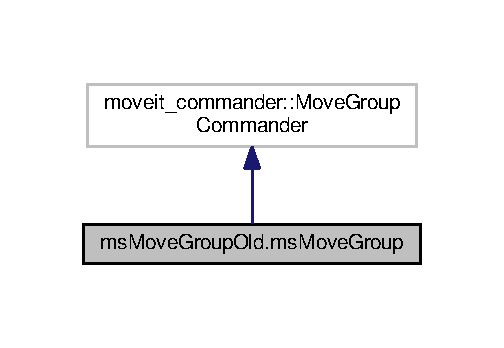
\includegraphics[width=242pt]{classmsMoveGroupOld_1_1msMoveGroup__inherit__graph}
\end{center}
\end{figure}


Collaboration diagram for ms\+Move\+Group\+Old.\+ms\+Move\+Group\+:\nopagebreak
\begin{figure}[H]
\begin{center}
\leavevmode
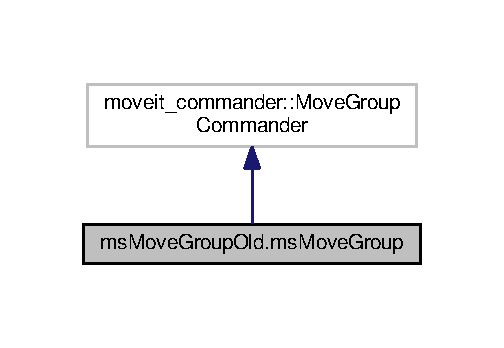
\includegraphics[width=242pt]{classmsMoveGroupOld_1_1msMoveGroup__coll__graph}
\end{center}
\end{figure}
\subsection*{Public Member Functions}
\begin{DoxyCompactItemize}
\item 
def {\bfseries \+\_\+\+\_\+init\+\_\+\+\_\+} (self, group\+Name)\hypertarget{classmsMoveGroupOld_1_1msMoveGroup_a98f3734be3cec4cbd132720b760adb93}{}\label{classmsMoveGroupOld_1_1msMoveGroup_a98f3734be3cec4cbd132720b760adb93}

\item 
def {\bfseries ms\+Plan} (self, position=None, posture=None, joint=None)\hypertarget{classmsMoveGroupOld_1_1msMoveGroup_a60fa838ffe63915bba5284bbb49f87b0}{}\label{classmsMoveGroupOld_1_1msMoveGroup_a60fa838ffe63915bba5284bbb49f87b0}

\item 
def {\bfseries ms\+Plan\+Way} (self, way\+Point, eef\+\_\+step=0.\+01, jump\+\_\+threshold=0.\+0, avoid\+\_\+collisions=True, move\+Success\+Ratio=0.\+5)\hypertarget{classmsMoveGroupOld_1_1msMoveGroup_adad133f1851a7bd595e769fc5fab4f6a}{}\label{classmsMoveGroupOld_1_1msMoveGroup_adad133f1851a7bd595e769fc5fab4f6a}

\item 
def {\bfseries ms\+Plan\+Shift} (self, vector\+List, reference\+Frame=None)\hypertarget{classmsMoveGroupOld_1_1msMoveGroup_ae737090ce31f5f2eaaad87920db649ec}{}\label{classmsMoveGroupOld_1_1msMoveGroup_ae737090ce31f5f2eaaad87920db649ec}

\item 
def {\bfseries ms\+Go} (self, position=None, posture=None, joint=None, is\+Wait\+Display\+Rviz=True)\hypertarget{classmsMoveGroupOld_1_1msMoveGroup_a9dbcc45f3641f8025d111f575b794351}{}\label{classmsMoveGroupOld_1_1msMoveGroup_a9dbcc45f3641f8025d111f575b794351}

\item 
def {\bfseries ms\+Get\+Current\+Pose} (self)\hypertarget{classmsMoveGroupOld_1_1msMoveGroup_a2a028894b0afe17eb4c45d1d54de2c02}{}\label{classmsMoveGroupOld_1_1msMoveGroup_a2a028894b0afe17eb4c45d1d54de2c02}

\item 
def {\bfseries ms\+Point\+To\+Position} (self, goal\+Position, arm\+Position, tip\+Direction\+Vector3=\mbox{[}0, base\+Open\+Vector=\mbox{[}0)\hypertarget{classmsMoveGroupOld_1_1msMoveGroup_aab7e2873cebb6612c1a306c4b2977dd2}{}\label{classmsMoveGroupOld_1_1msMoveGroup_aab7e2873cebb6612c1a306c4b2977dd2}

\item 
def {\bfseries ms\+Pick} (self, object\+Id, gripping\+Joint\+Angle, openning\+Joint\+Angle, object\+Point=None, grip\+Posture=None, grip\+Position=\mbox{[}0, to\+Grip\+Move\+Vector=\mbox{[}0, to\+Retreat\+Move\+Vector=\mbox{[}0, try\+Num=2)\hypertarget{classmsMoveGroupOld_1_1msMoveGroup_a5859c9d9983ec4e03d57e56f348d4989}{}\label{classmsMoveGroupOld_1_1msMoveGroup_a5859c9d9983ec4e03d57e56f348d4989}

\item 
def {\bfseries ms\+Place} (self, object\+Id, openning\+Joint\+Angle, place\+Position, to\+Place\+Move\+Vector=\mbox{[}0, to\+Retreat\+Move\+Vector=\mbox{[}0)\hypertarget{classmsMoveGroupOld_1_1msMoveGroup_a366b600e9d9d02582df541d94734048d}{}\label{classmsMoveGroupOld_1_1msMoveGroup_a366b600e9d9d02582df541d94734048d}

\item 
def {\bfseries make\+Gripper\+Posture} (self, joint\+Angle)\hypertarget{classmsMoveGroupOld_1_1msMoveGroup_a18bb8b3ececb662a7580203354378e94}{}\label{classmsMoveGroupOld_1_1msMoveGroup_a18bb8b3ececb662a7580203354378e94}

\item 
def {\bfseries make\+Gripper\+Translation} (self, min\+\_\+dist, desired, vector)\hypertarget{classmsMoveGroupOld_1_1msMoveGroup_a933940b988af395523e3a9121d0aaffb}{}\label{classmsMoveGroupOld_1_1msMoveGroup_a933940b988af395523e3a9121d0aaffb}

\item 
def {\bfseries make\+Arm\+Poses} (self, position, option=\char`\"{}R\+I\+NG\char`\"{})\hypertarget{classmsMoveGroupOld_1_1msMoveGroup_ae4f947f53bd380cd899593735f11bea6}{}\label{classmsMoveGroupOld_1_1msMoveGroup_ae4f947f53bd380cd899593735f11bea6}

\end{DoxyCompactItemize}
\subsection*{Public Attributes}
\begin{DoxyCompactItemize}
\item 
{\bfseries pick\+Number}\hypertarget{classmsMoveGroupOld_1_1msMoveGroup_ac350a567d795bb726bacb9c62d7877ea}{}\label{classmsMoveGroupOld_1_1msMoveGroup_ac350a567d795bb726bacb9c62d7877ea}

\item 
{\bfseries place\+Number}\hypertarget{classmsMoveGroupOld_1_1msMoveGroup_ad6352b86f617980bb947f907ac2c5c78}{}\label{classmsMoveGroupOld_1_1msMoveGroup_ad6352b86f617980bb947f907ac2c5c78}

\item 
{\bfseries tfg}\hypertarget{classmsMoveGroupOld_1_1msMoveGroup_a90b06e576bbd2feea38d771a85357610}{}\label{classmsMoveGroupOld_1_1msMoveGroup_a90b06e576bbd2feea38d771a85357610}

\end{DoxyCompactItemize}


The documentation for this class was generated from the following file\+:\begin{DoxyCompactItemize}
\item 
ms\+Move\+Group\+Old.\+py\end{DoxyCompactItemize}

\hypertarget{classmsMath_1_1onlineStandardDeviations}{}\section{ms\+Math.\+online\+Standard\+Deviations Class Reference}
\label{classmsMath_1_1onlineStandardDeviations}\index{ms\+Math.\+online\+Standard\+Deviations@{ms\+Math.\+online\+Standard\+Deviations}}
\subsection*{Public Member Functions}
\begin{DoxyCompactItemize}
\item 
def {\bfseries \+\_\+\+\_\+init\+\_\+\+\_\+} (self)\hypertarget{classmsMath_1_1onlineStandardDeviations_aefffd5741b605cea400ef347f7710142}{}\label{classmsMath_1_1onlineStandardDeviations_aefffd5741b605cea400ef347f7710142}

\item 
def {\bfseries input} (self, data)\hypertarget{classmsMath_1_1onlineStandardDeviations_a45b2579ea416b3b7f01d7c675bea291f}{}\label{classmsMath_1_1onlineStandardDeviations_a45b2579ea416b3b7f01d7c675bea291f}

\item 
def {\bfseries get\+Average} (self)\hypertarget{classmsMath_1_1onlineStandardDeviations_a60b2e5b01196a83f22fa952a81cedac1}{}\label{classmsMath_1_1onlineStandardDeviations_a60b2e5b01196a83f22fa952a81cedac1}

\item 
def {\bfseries get\+Variance} (self)\hypertarget{classmsMath_1_1onlineStandardDeviations_ac725aac7593b0eb31bb109c7fdfc86fc}{}\label{classmsMath_1_1onlineStandardDeviations_ac725aac7593b0eb31bb109c7fdfc86fc}

\item 
def {\bfseries get\+Standard\+Deviation} (self)\hypertarget{classmsMath_1_1onlineStandardDeviations_a67025340b07659590de7e309bc5e1320}{}\label{classmsMath_1_1onlineStandardDeviations_a67025340b07659590de7e309bc5e1320}

\item 
def {\bfseries get\+Data\+Num} (self)\hypertarget{classmsMath_1_1onlineStandardDeviations_a419ce39e6c7af2b2b612371e05ed3d9f}{}\label{classmsMath_1_1onlineStandardDeviations_a419ce39e6c7af2b2b612371e05ed3d9f}

\item 
def {\bfseries get\+Result} (self)\hypertarget{classmsMath_1_1onlineStandardDeviations_aa2cd46633ff8694408ed62a03c526576}{}\label{classmsMath_1_1onlineStandardDeviations_aa2cd46633ff8694408ed62a03c526576}

\end{DoxyCompactItemize}
\subsection*{Public Attributes}
\begin{DoxyCompactItemize}
\item 
{\bfseries average}\hypertarget{classmsMath_1_1onlineStandardDeviations_a536006417b4620f934f6297f3ef19be5}{}\label{classmsMath_1_1onlineStandardDeviations_a536006417b4620f934f6297f3ef19be5}

\item 
{\bfseries mn}\hypertarget{classmsMath_1_1onlineStandardDeviations_a90e0aa23587900677755e52e99147bac}{}\label{classmsMath_1_1onlineStandardDeviations_a90e0aa23587900677755e52e99147bac}

\item 
{\bfseries data\+Num}\hypertarget{classmsMath_1_1onlineStandardDeviations_aaa8088f76ceb012c28e33973c2d532ec}{}\label{classmsMath_1_1onlineStandardDeviations_aaa8088f76ceb012c28e33973c2d532ec}

\end{DoxyCompactItemize}


The documentation for this class was generated from the following file\+:\begin{DoxyCompactItemize}
\item 
ms\+Math.\+py\end{DoxyCompactItemize}

\hypertarget{classmsTfGetter_1_1tfGetter}{}\section{ms\+Tf\+Getter.\+tf\+Getter Class Reference}
\label{classmsTfGetter_1_1tfGetter}\index{ms\+Tf\+Getter.\+tf\+Getter@{ms\+Tf\+Getter.\+tf\+Getter}}


rosのtfモジュールを自分用にわかりやすくラッパーしたもの~\newline
 と言っても、名前をまとめてlistenerとbroadcasterをまとめたもの  


\subsection*{Public Member Functions}
\begin{DoxyCompactItemize}
\item 
def \hyperlink{classmsTfGetter_1_1tfGetter_a576aeceb58ed338d02d4457b51ec7158}{\+\_\+\+\_\+init\+\_\+\+\_\+} (self)\hypertarget{classmsTfGetter_1_1tfGetter_a576aeceb58ed338d02d4457b51ec7158}{}\label{classmsTfGetter_1_1tfGetter_a576aeceb58ed338d02d4457b51ec7158}

\begin{DoxyCompactList}\small\item\em tfとtf2のクラスを初期化~\newline
 0.\+5sのsleepを含む \end{DoxyCompactList}\item 
def {\bfseries get} (self)\hypertarget{classmsTfGetter_1_1tfGetter_a2fff7638f57fc7b015edce329565f462}{}\label{classmsTfGetter_1_1tfGetter_a2fff7638f57fc7b015edce329565f462}

\item 
def \hyperlink{classmsTfGetter_1_1tfGetter_a2197923dada642c3d44df94990503e9a}{broadcast\+Tf} (self, transform\+Stamped)
\begin{DoxyCompactList}\small\item\em 値のtfをbroadcastする \end{DoxyCompactList}\item 
def \hyperlink{classmsTfGetter_1_1tfGetter_a82484ce686977bd9e1d3ffa2e3de5aee}{broadcast\+Static\+Tf} (self, transform\+Stamped)
\begin{DoxyCompactList}\small\item\em 値が永続するtfをbroadcastする \end{DoxyCompactList}\item 
def \hyperlink{classmsTfGetter_1_1tfGetter_aadb0e5d08e8c080fed67e1f7afe26931}{look\+Transform} (self, from\+Tf\+Name, to\+Tf\+Name)
\begin{DoxyCompactList}\small\item\em from\+Tf\+Nameからみたto\+Tf\+Nameの状態を得る ~\newline
 timeoutは0.05s \end{DoxyCompactList}\item 
def \hyperlink{classmsTfGetter_1_1tfGetter_a170eb4a51944de61b2bfecff14df4a9a}{get\+Pose\+From\+Tf} (self, from\+Tf\+Name, pose\+Stamp)
\begin{DoxyCompactList}\small\item\em from\+Tf\+Nameの基準座標系から見た、pose\+Stamp.\+header.\+frame\+\_\+idの座標系で表されるpose\+Stamp.\+poseの姿勢を取得する \end{DoxyCompactList}\end{DoxyCompactItemize}


\subsection{Detailed Description}
rosのtfモジュールを自分用にわかりやすくラッパーしたもの~\newline
 と言っても、名前をまとめてlistenerとbroadcasterをまとめたもの 

\begin{DoxyAuthor}{Author}
sugino 
\end{DoxyAuthor}
\begin{DoxyVersion}{Version}
1.\+1 
\end{DoxyVersion}
\begin{DoxySince}{Since}
2018/12/21 
\end{DoxySince}


\subsection{Member Function Documentation}
\index{ms\+Tf\+Getter\+::tf\+Getter@{ms\+Tf\+Getter\+::tf\+Getter}!broadcast\+Static\+Tf@{broadcast\+Static\+Tf}}
\index{broadcast\+Static\+Tf@{broadcast\+Static\+Tf}!ms\+Tf\+Getter\+::tf\+Getter@{ms\+Tf\+Getter\+::tf\+Getter}}
\subsubsection[{\texorpdfstring{broadcast\+Static\+Tf(self, transform\+Stamped)}{broadcastStaticTf(self, transformStamped)}}]{\setlength{\rightskip}{0pt plus 5cm}def ms\+Tf\+Getter.\+tf\+Getter.\+broadcast\+Static\+Tf (
\begin{DoxyParamCaption}
\item[{}]{self, }
\item[{}]{transform\+Stamped}
\end{DoxyParamCaption}
)}\hypertarget{classmsTfGetter_1_1tfGetter_a82484ce686977bd9e1d3ffa2e3de5aee}{}\label{classmsTfGetter_1_1tfGetter_a82484ce686977bd9e1d3ffa2e3de5aee}


値が永続するtfをbroadcastする 


\begin{DoxyParams}{Parameters}
{\em transform\+Stamped} & = tfに上げる\+Transform\+Stamped \\
\hline
\end{DoxyParams}
\index{ms\+Tf\+Getter\+::tf\+Getter@{ms\+Tf\+Getter\+::tf\+Getter}!broadcast\+Tf@{broadcast\+Tf}}
\index{broadcast\+Tf@{broadcast\+Tf}!ms\+Tf\+Getter\+::tf\+Getter@{ms\+Tf\+Getter\+::tf\+Getter}}
\subsubsection[{\texorpdfstring{broadcast\+Tf(self, transform\+Stamped)}{broadcastTf(self, transformStamped)}}]{\setlength{\rightskip}{0pt plus 5cm}def ms\+Tf\+Getter.\+tf\+Getter.\+broadcast\+Tf (
\begin{DoxyParamCaption}
\item[{}]{self, }
\item[{}]{transform\+Stamped}
\end{DoxyParamCaption}
)}\hypertarget{classmsTfGetter_1_1tfGetter_a2197923dada642c3d44df94990503e9a}{}\label{classmsTfGetter_1_1tfGetter_a2197923dada642c3d44df94990503e9a}


値のtfをbroadcastする 


\begin{DoxyParams}{Parameters}
{\em transform\+Stamped} & = tfに上げる\+Transform\+Stamped \\
\hline
\end{DoxyParams}
\index{ms\+Tf\+Getter\+::tf\+Getter@{ms\+Tf\+Getter\+::tf\+Getter}!get\+Pose\+From\+Tf@{get\+Pose\+From\+Tf}}
\index{get\+Pose\+From\+Tf@{get\+Pose\+From\+Tf}!ms\+Tf\+Getter\+::tf\+Getter@{ms\+Tf\+Getter\+::tf\+Getter}}
\subsubsection[{\texorpdfstring{get\+Pose\+From\+Tf(self, from\+Tf\+Name, pose\+Stamp)}{getPoseFromTf(self, fromTfName, poseStamp)}}]{\setlength{\rightskip}{0pt plus 5cm}def ms\+Tf\+Getter.\+tf\+Getter.\+get\+Pose\+From\+Tf (
\begin{DoxyParamCaption}
\item[{}]{self, }
\item[{}]{from\+Tf\+Name, }
\item[{}]{pose\+Stamp}
\end{DoxyParamCaption}
)}\hypertarget{classmsTfGetter_1_1tfGetter_a170eb4a51944de61b2bfecff14df4a9a}{}\label{classmsTfGetter_1_1tfGetter_a170eb4a51944de61b2bfecff14df4a9a}


from\+Tf\+Nameの基準座標系から見た、pose\+Stamp.\+header.\+frame\+\_\+idの座標系で表されるpose\+Stamp.\+poseの姿勢を取得する 


\begin{DoxyParams}{Parameters}
{\em from\+Tf\+Name(\+String)} & = 取得したい値の基準座標系のtf \\
\hline
{\em pose\+Stamp(\+Pose\+Stamped)} & = 取得したい座標系の情報を含んだ姿勢~\newline
 pose\+Stamp.\+header.\+stampが空なら、現時刻を取得 \\
\hline
\end{DoxyParams}
\begin{DoxyReturn}{Returns}
成功 = Transform\+Stamped 

失敗 = False 
\end{DoxyReturn}
\index{ms\+Tf\+Getter\+::tf\+Getter@{ms\+Tf\+Getter\+::tf\+Getter}!look\+Transform@{look\+Transform}}
\index{look\+Transform@{look\+Transform}!ms\+Tf\+Getter\+::tf\+Getter@{ms\+Tf\+Getter\+::tf\+Getter}}
\subsubsection[{\texorpdfstring{look\+Transform(self, from\+Tf\+Name, to\+Tf\+Name)}{lookTransform(self, fromTfName, toTfName)}}]{\setlength{\rightskip}{0pt plus 5cm}def ms\+Tf\+Getter.\+tf\+Getter.\+look\+Transform (
\begin{DoxyParamCaption}
\item[{}]{self, }
\item[{}]{from\+Tf\+Name, }
\item[{}]{to\+Tf\+Name}
\end{DoxyParamCaption}
)}\hypertarget{classmsTfGetter_1_1tfGetter_aadb0e5d08e8c080fed67e1f7afe26931}{}\label{classmsTfGetter_1_1tfGetter_aadb0e5d08e8c080fed67e1f7afe26931}


from\+Tf\+Nameからみたto\+Tf\+Nameの状態を得る ~\newline
 timeoutは0.05s 


\begin{DoxyParams}{Parameters}
{\em from\+Tf\+Name(\+String)} & = 基準座標となる\+Tfの名前 \\
\hline
{\em to\+Tf\+Name(\+String)} & = 取得対象となる\+Tfの名前 \\
\hline
\end{DoxyParams}
\begin{DoxyReturn}{Returns}
成功 = Transform\+Stamped 

失敗or\+Timeout = False 
\end{DoxyReturn}


The documentation for this class was generated from the following file\+:\begin{DoxyCompactItemize}
\item 
ms\+Tf\+Getter.\+py\end{DoxyCompactItemize}

%--- End generated contents ---

% Index
\backmatter
\newpage
\phantomsection
\clearemptydoublepage
\addcontentsline{toc}{chapter}{Index}
\printindex

\end{document}
